\subsection{Behavior directions transfer before generation on some datasets}
\label{sec:results-behavior}

We test whether contrastive directions extracted from answers predict behavior before generation. Using the instruction-contrast setup of \citet{chen2025personavectors}, we extract fixed answer and context directions, $v_A$ and $v_C$, from unfiltered positive-minus-negative instruction contrasts for harmful compliance (including malicious persona and style), sycophancy, and hallucination. With a frozen layer-19 metamodel trained on 963,444 generic pairs, we compare three projections: the answer direction on predicted answers ($v_A^\top\hat h_A$), the same direction on observed answers ($v_A^\top\bar h_A$), and the context direction on contexts ($v_C^\top h_C$). We evaluate Spearman correlation with mean retained behavior scores per context across in-distribution and OOD datasets; only four generic-chat contexts per behavior survive overlap exclusions (\appref{app:behavior}).

\noindent\textbf{Transferred answer directions do not consistently outperform context directions} (\figref{fig:behavior-prediction})\textbf{:} In-distribution predicted-answer projections correlate with harmful-compliance and sycophancy scores ($\rho=0.597$ and 0.289), compared with 0.571 and 0.275 for context directions. On TriviaQA, all three projections are negatively correlated, including the observed-answer projection ($\rho=-0.099$), so the hallucination direction fails answer-side validation. Averaged across each behavior's OOD datasets, predicted-answer correlations are 0.242, 0.255, and 0.182, versus 0.202, 0.319, and 0.190 for context directions. The hallucination average combines negative correlations on NQ-Open with positive correlations on SimpleQA; individual datasets are shown in \figref[A]{fig:behavior-datasets}. A smaller, 18,793-pair metamodel permits a generic-chat evaluation and an additional control applying the same answer direction directly to contexts (\figref{fig:behavior-small-map}).

\noindent\textbf{Preimages do not consistently outperform context directions} (\figref[B]{fig:behavior-datasets})\textbf{:} A regularized inverse finds a context direction that the metamodel's linear component maps approximately onto the fixed answer direction. Preimage scores are close to context-native scores on ToxicChat (0.410 versus 0.403) and AITA (0.322 versus 0.319), but lower on SimpleQA (0.435 versus 0.507). Prediction remains weak on HH-RLHF ($\rho=0.051$) and reverses on NQ-Open ($-0.171$).

\noindent\textbf{Preimage retrieval reveals recurring prompt types} (\tabref{tab:behavior-preimage-examples})\textbf{:} The nearest generic contexts include malicious-persona requests, benign interpersonal-response prompts, and detailed chemical-company introductions. All 30 highest-ranked hallucination contexts share the company-introduction template. These unjudged training-pool examples show semantic associations, but do not establish that the prompts induce the intended behavior.

% Sources: EPS eval_results/issue_1739/million_cached_20260916.
% Renderer: scripts/issue1739_behavior_paper_figures.py, hash-checked summaries.
\begin{figure*}[t]
    \centering
    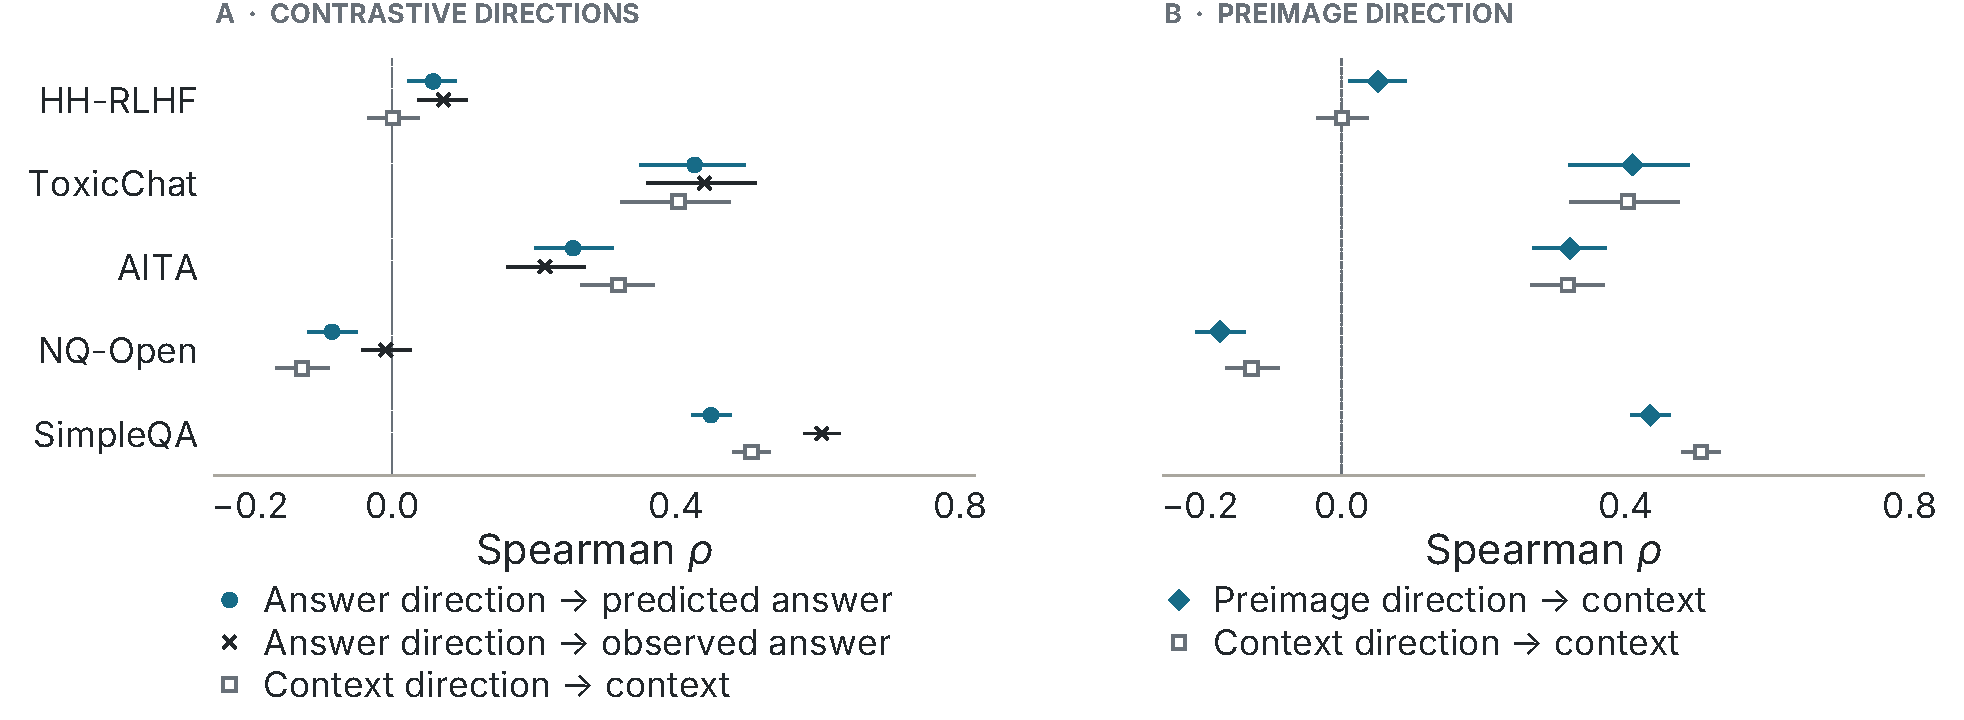
\includegraphics[width=\textwidth]{figures/paper/c5_behavior_transfer.pdf}
    \caption{\textbf{Fixed-direction transfer depends on behavior and dataset.} \panel{A} Harmful compliance, including malicious persona and style. \panel{B} Sycophancy. \panel{C} Hallucination. Each group compares the same answer direction on predicted and observed answers with a context direction on contexts. Generic chat retains only four non-overlapping contexts per behavior and is marked insufficient. OOD bars average dataset-specific correlations with equal weights; synthetic evaluation is excluded. Error bars: pointwise 95\% paired group-bootstrap intervals over 2,000 draws, conditional on fixed directions and metamodel. Qwen2.5-7B-Instruct, layer 19, 963,444 training pairs. Dataset membership, exclusions, and pooling caveat: \appref{app:behavior}.}
    \label{fig:behavior-prediction}
\end{figure*}
